% This paper is Copyright © Graeme Andrew Stewart, Sam Skipsey, 
% authors, 2025.
% Licensed under Creative Commons Attribution 4.0 International (CC BY 4.0), see LICENSE

\documentclass{webofc}
\usepackage{graphicx} % Required for inserting images
\graphicspath{{figures/}}
\usepackage{subcaption}
\usepackage[varg]{txfonts}
\usepackage[utf8]{inputenc}

% Workaround for arXiv, start with "finalizecache" then switch to "frozencache"
\usepackage[finalizecache,cachedir=.]{minted}
% \usepackage[frozencache,cachedir=.]{minted}

\usepackage{natbib}
\usepackage{hyperref}
\usepackage{enumitem} % This seems to cause nested itemize lists to break...?

% For draftversion
\usepackage{lineno}
\linenumbers

\title{Julia in HEP}

\author{\firstname{Graeme Andrew} \lastname{Stewart}\inst{1}\fnsep\thanks{\email{graeme.andrew.stewart@cern.ch}} \and
\firstname{Alexander} \lastname{Moreno Briceño}\inst{2} \and
\firstname{Philippe} \lastname{Gras}\inst{3} \and
\firstname{Benedikt} \lastname{Hegner}\inst{1} \and
\firstname{Uwe} \lastname{Hernandez Acosta}\inst{4,5} \and
\firstname{Tamas} \lastname{Gal}\inst{6} \and
\firstname{Jerry} \lastname{Ling}\inst{7} \and
\firstname{Pere} \lastname{Mato}\inst{1} \and
\firstname{Mikhail} \lastname{Mikhasenko}\inst{8} \and
\firstname{Oliver} \lastname{Schulz}\inst{9} \and
\firstname{Sam} \lastname{Skipsey}\inst{10}
% etc.
}

\institute{CERN, Esplanade des Particules 1, Geneva, Switzerland
\and
Universidad Antonio Nariño, Ibagué, Colombia
\and
IRFU, CEA, Université Paris-Saclay, Gif-sur-Yvette, France
\and
Center for Advanced Systems Understanding, Görlitz, Germany
\and
Helmholtz-Zentrum Dresden-Rossendorf, Dresden, Germany
\and
Erlangen Centre for Astroparticle Physics, Friedrich-Alexander-Universität, Erlangen-Nürnberg, Germany
\and
Laboratory for Particle Physics and Cosmology, Harvard University, Cambridge, MA, USA
\and
Ruhr Universität Bochum, Bochum, Germany
\and
Max-Planck-Institut für Physik, Munich, Germany
\and
School of Physics \& Astronomy, University of Glasgow, Glasgow, United Kingdom, G12 8QQ
}


\abstract{%
Julia is a mature general-purpose programming language, with a large ecosystem
of libraries and more than 10000 third-party packages, which specifically
targets scientific computing. As a language, Julia is as dynamic, interactive,
and accessible as Python with NumPy, but achieves run-time performance on par
with C/C++. In this paper, we describe the state of adoption of Julia in HEP,
where momentum has been gathering over a number of years.

HEP-oriented Julia packages can, via \texttt{UnROOT.jl}, already read HEP's
major file formats, including TTree and RNTuple formats. Interfaces to some of
HEP's major software packages, such as through \texttt{Geant4.jl}, are available
too. Jet reconstruction algorithms in Julia show excellent performance. A number
of full HEP analyses have been performed in Julia.

We show how, as the support for HEP has matured, developments have benefited
from Julia's core design choices, which makes reuse from and integration with
other packages easy. In particular, libraries developed outside HEP for
plotting, statistics, fitting, and scientific machine learning are extremely
useful.

We believe that the powerful combination of flexibility and speed, the wide
selection of scientific programming tools, and support for all modern
programming paradigms and tools, make Julia the ideal choice for a future
language in HEP.}

\begin{document}

\maketitle

\section{Programming Languages in High-Energy Physics}
\label{sec:introduction}

\subsection{HEP Needs}

High-energy physics (HEP) is a large field, consisting of tens of thousands of
researchers, almost all of whom will need to interact with software and
contribute to software projects during their careers~\cite{2024EPJWC.29505023M}.
It is also one of the biggest, if not the biggest, generators of scientific
datasets today, with exabytes of storage used by the LHC
experiments~\cite{Collaboration:2904204}. This data is processed by a huge
corpus of software, estimated to be many tens of millions of lines in
C++~\cite{hsfcwp}.

This brings a challenge for HEP software. From the point of view of \emph{code
efficiency} we require fast and efficient execution, high throughput, and
scalability at large computer centres and across distributed infrastructures.
Considering \emph{human efficiency} we would like a low barrier to entry for
newcomers, the ability to prototype code rapidly, a broad ecosystem of well
maintained packages, and excellent tooling for developers. These features are
needed to make software able to deal efficiently with huge datasets, as well as
accessible to a large group of developers.

\subsection{From Fortran to the C++/Python Era}

In response to changing technology, and the needs of the field, the programming
languages that are dominant in the field have evolved over time.
From~\cite{pivarski2022} we can identify three major shifts as seen in
\ref{fig:hep-languages}. 

\begin{figure}[htbp]
    \begin{center}
        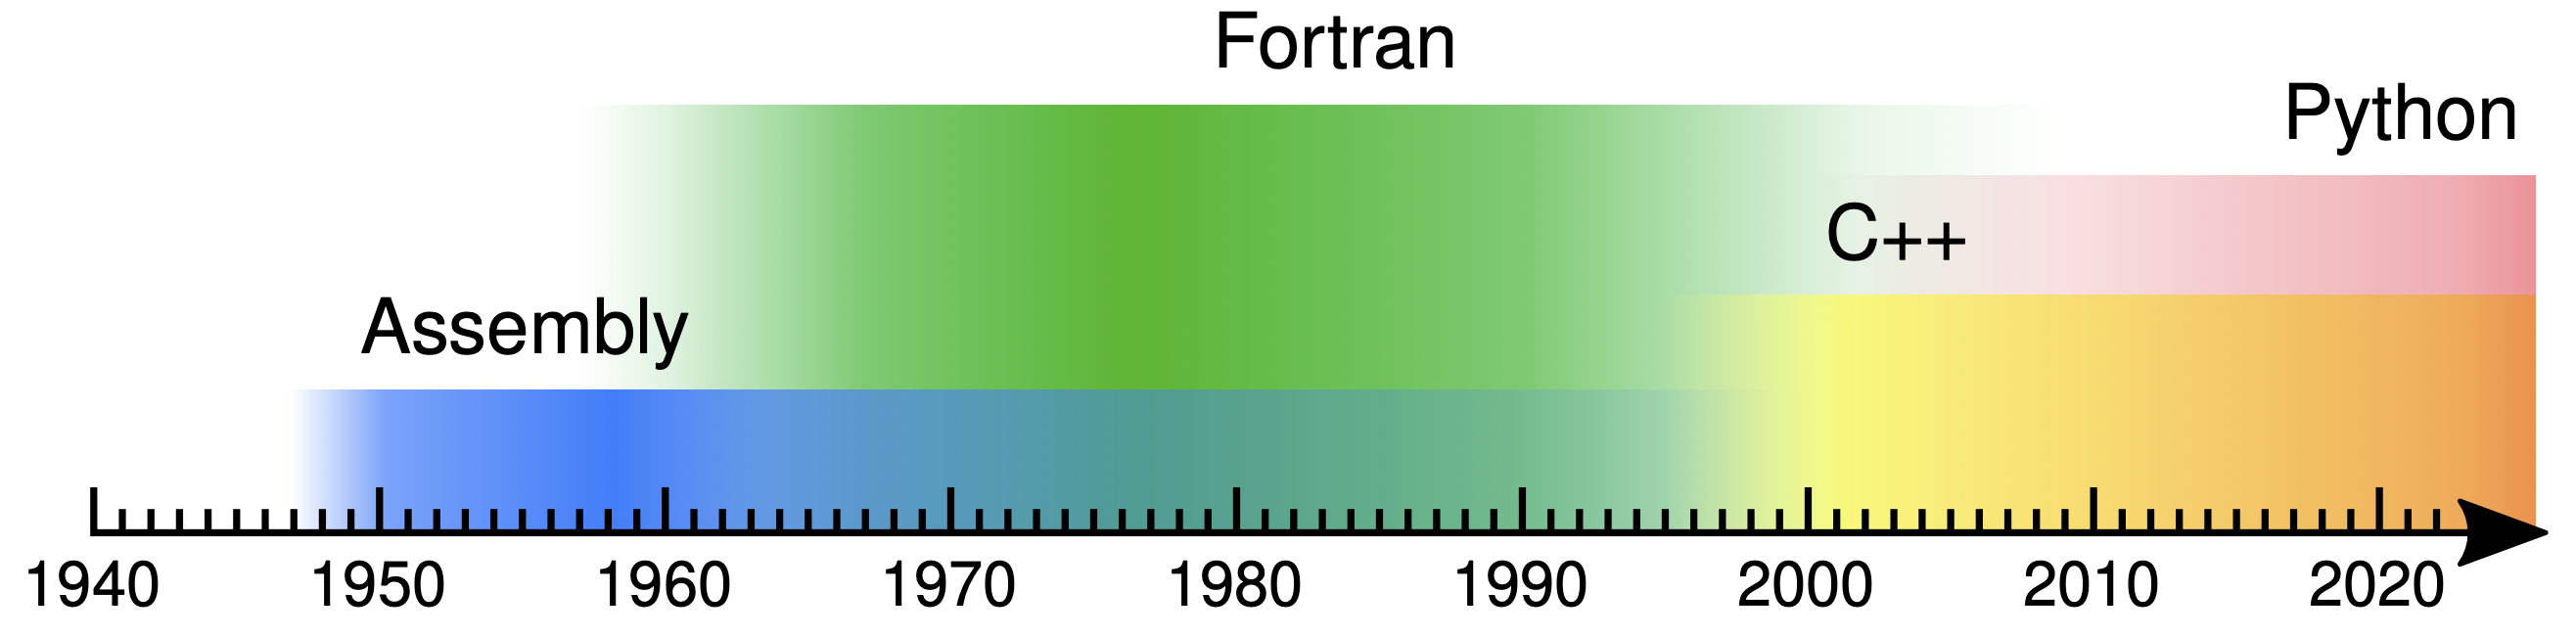
\includegraphics[width=0.7\textwidth]{hep-programming-languages.png}
        \caption{Illustrative cartoon of major shifts in HEP programming languages, from~\cite{pivarski2022}.}
        \label{fig:hep-languages}
    \end{center}
\end{figure}

\begin{description}
    \item[From assembler to Fortran] As computers developed from early
    specialised behemoths, with barely an operating system, improved programming
    languages became available. For technical computing Fortran was the most
    effective language and HEP quickly adopted it as it brought a much improved
    syntax, as well as hardware portability.
    \item[From Fortan to C++] Although Fortran had many advantages, HEP had to
    develop language extensions to introduce concepts such as more advanced data
    structures~\cite{Zoll:2296399}. A language which offered native object
    orientation was an attractive choice. In addition, the gap afforded by the
    end of the LEP accelerator and the construction of the LHC allowed the field
    to afford the time for a major language shift.
    \item[The rise of Python] Python earned a well deserved reputation as an
    excellent language for programming efficiency, and also gained ground
    through being the de facto interface to many machine learning libraries. It
    has become widely used in HEP as a compliment to C++.
\end{description}

The current situation for HEP is that C++ and Python are now both widely used,
with each bringing specific advantages, as well as drawbacks. Good C++ excels at
runtime efficiency, but is a difficult language to learn and master as well as
suffering from memory safety issues and being difficult to compose. Python is
expressive, much easier to work with, is safer with memory and composes better
(duck typing). However, it is very slow compared to C++, so not suitable for
high throughput computing.

As noted in~\cite{eschle2023potential}, using two languages is not ideal: it
increases the required expertise, necessitates reimplementation of code for
performance, and reduces code reusability.

\section{Julia}

\subsection{Julia's Motivations}

The Julia programming language was announced in 2012 with a blog post entitled
``Why We Created Julia''~\cite{why-create-julia}. This document lists a series of
ambitious goals for the language, and represents a view into the core
developers' mindset formalised in a later
paper~\cite{bib:julia_freshapproach,10.1145/3276490}.

Julia provides a syntax as productive as Python, especially for numerical work,
whilst leveraging JAOT\footnote{Just-Ahead-Of-Time} compilation to provide speed
similar to compiled, statically typed languages like C and Rust. It utilises
type inference to allow coding in a ``gradually typed'', generic programming
style, although the language will always track types for performance behind the
scenes, and types can be specified explicitly if required. Like MatLab and
Fortran, Julia's native operations and type system support arrays as first-class
entities, of any dimension, allowing array-oriented code to be both productively
generated, and efficiently executed, with operations naturally ``broadcasted''
element- or dimension-wise. This allows Julia to also be effective for writing
linear algebra heavy code. In addition, influence from the R community provides
a wealth of statistical packages, and an R-flavoured approach to plots and
visualisation. Of course, as with most languages of the 21st century, Julia is a
fully open-source language, with its entire codebase freely available (and
almost all of it written in Julia itself).

\subsection{Julia in Practice}

Julia's syntax is familiar to programmers conversant with programming performant
code in Python with NumPy, except that whitespace is not syntactically relevant
(blocks end with \texttt{end}).

For example, the listing in Figure~\ref{code:madelbrot} shows some toy code to
generate a grayscale image of the famous Mandelbröt set.

\begin{figure}[!ht]
\centering
\begin{minted}[linenos]{julia}
using Images

function mandel(z)
    c = z
    maxiter = 80
    for n = 1:maxiter
        if abs2(z) > 4
            return n-1
        end
        z = z^2 + c
    end
    maxiter
end

set = [ mandel(complex(r,i)) for i=-1.:.01:1., r=-2.0:.01:0.5 ]
img = Gray.(set ./ 80)
\end{minted}
\caption{Julia implementation of the Mandelbr\"{o}t set}
\label{code:madelbrot}
\end{figure}

Here we demonstrate importing of packages (line 1), function declaration with
implicit types and explicit loop and branch constructs, implicit loops via
``comprehensions'' to generate a  value for every point in an implicitly defined
array, and, finally, transparent broadcasting of operations over that array
(both the function call to Gray, and the division operation are distributed over
the whole array). Unlike Python, explicit loops are optimised efficiently, and
are no slower than comprehensions or ``functional-style'' iterators (which are
also supported by Julia).

%Tooling and ecosystem.
As with other languages of the 2010s, Julia comes with a set of tools for
managing development environments beyond the interpreter.

\texttt{juliaup} allows seamless management of multiple Julia releases on the same
machine, including tracking particular patch releases, and choosing the system
default.

The integrated package management in Julia -- via the Pkg library, or a
sub-environment within a Julia REPL accessed by pressing '$]$', tracks and
maintains the dependency graph of a Julia project. State is entirely stored
within two human-readable files - \texttt{Project.toml} (which represents the direct
dependencies of the project) and \texttt{Manifest.toml} (which preserves the exact
resulting environment, including secondary dependencies and exact versions).
The user of a Julia codebase can easily reproduce the exact environment used by
the codebase as long as these files are provided.

The Julia Package ``General Registry'' indexes packages and their releases, and
(as with other languages such as Rust and Javascript) relies on a public index
hosted on GitHub (with off-GitHub backups). A help environment, accessed by
\texttt{?} on an empty line of the REPL, allows interactive help on any keyword
or symbol known to the REPL; it is trivial to add documentation to a function or
type by simply prepending its definition with a triple-quoted string -- this is
immediately available to the help environment.

Leveraging the fact that Julia is JAOT-compiled, and that this allows its entire
standard library to be written in idiomatic Julia, the REPL also provides a
series of powerful macro utilities for inspecting the byte- and machine-code
generated for a given expression (\verb$@code_lowered$, \verb$@code_native$) and
for locating and displaying the source code for any function in the current
namespace, including from the standard library (\verb$@less$), as well as other
introspection tools. Profiling of code in the REPL is similarly directly
supported via macros (\verb$@benchmark$...), which provide detailed performance
sampling, including execution time distributions and GC invocations. Extended
introspection and profiling tools are also available in optional packages, such
as \texttt{About.jl}, which can provide information on memory layout of
datatypes and thread safety of functions.

A well-supported VSCode extension is available for the language, which also
supports the standard LSP allowing it to support development in other editors.
This includes the usual benefits of code completion (and Unicode completion for
non-ASCII characters), linting, highlighting and so on.

Finally, Julia is one of the founding languages supported by Jupyter - being the
``Ju'' in the portmanteau - and also provides other native notebook
implementations such as Pluto.jl. 

\subsection{Key Design Features for Performance}

Type system.

Multiple dispatch.

\section{Julia for Scientific Computing}

General adoption:~\cite{perkel-julia-science}.

GPU programming.

Some HPC codes.

\section{Julia in HEP}

\subsection{Challenges}

What does HEP need from its computing?

Cite some general overviews:~\cite{Stanitzki:2020bnx,eschle2023potential}.

\subsection{HEP Data Formats}

We can read that data... UpROOT.jl. EDM4hep.jl.

\subsection{Event Generators}

The numerical calculation of amplitudes for hard scattering processes and Monte
Carlo event generation plays a fundamental role in high-energy physics analysis
workflows, with a long history (\cite{campbell2024event}). Consequently,
integrating various aspects of physics models with specialized numerical
algorithms in a high-performance computing environment is recognized as one
major challenge in HEP software development for future HEP experiments
(\cite{HEPSoftwareFoundation:2017ggl, HSFPhysicsEventGeneratorWG:2020gxw,
HSFPhysicsEventGeneratorWG:2021xti}) and beyond.

With the open-source framework \texttt{QuantumElectrodynamics.jl}
\cite{qedjl-github}, we take the first steps in exploring how the Julia
programming language can address these challenges. Specifically, our framework
facilitates the numerical calculation of scattering amplitudes and the
implementation of Monte Carlo event generation within the domain of perturbative
and strong-field quantum electrodynamics (cf. \cite{Fedotov:2022ely}). The
overall structure of the framework is unified through interfaces defined in
\texttt{QEDbase.jl}, which provides standardized representations for fundamental
mathematical objects such as four-momenta, bi-spinors, and phase space points.
Additionally, these interfaces extend to the configuration entities like
scattering processes, computational models, and phase space layouts. Further
interfaces are provided for computable quantities, such as differential
cross-sections, and various samplers for Monte Carlo event generation. Here,
Julia’s multiple dispatch mechanism proves particularly powerful, allowing
different implementations to be seamlessly integrated without explicitly
specifying types within the interface definitions. Moreover, the domain-specific
language facilitated by these interfaces—covering elements such as processes,
models, and phase space layouts—combined with multiple dispatch enables the
straightforward incorporation of analytical formulas whenever they are
available. This typically reduces to implementing a single method for a specific
function signature.

Beyond its interface definitions, \texttt{QuantumElectrodynamics.jl} provides
concrete implementations for all major components: \texttt{QEDcore.jl} handles
the fundamental mathematical structures, \texttt{QEDprocesses.jl} computes
differential cross sections, and \texttt{QEDevents.jl} offers different samplers
for event generation. The \texttt{QEDFeynmanDiagrams.jl} package, as part of
\texttt{QEDprocesses.jl}, facilitates the calculation of scattering amplitudes
for arbitrary QED processes by leveraging Julia's metaprogramming and code
generation capabilities. Built on top of \texttt{ComputableDAGs.jl}, the
generated code can be directly analysed and manipulated within Julia itself,
even without leaving the session. This enables meta-optimizations based on
domain-specific knowledge, such as recognizing patterns in Feynman diagrams and
exploiting mathematical properties like distributivity.

Finally, by leveraging multiple dispatch and various array abstractions from the
Julia ecosystem—such as \texttt{CUDA.jl} and \texttt{AMDGPU.jl}—the generated
code can be seamlessly compiled and executed on GPUs in addition to CPUs,
without requiring any modifications to its underlying structure. While some
framework components are still under development and will be further extended to
address broader challenges in high-energy physics, the initial structures
demonstrate great potential. The modular design, combined with Julia's
capabilities, has the potential to contribute to future developments in
numerical calculations and event generation within HEP.


\subsection{Simulation}

Detector simulation is a crucial component of every High Energy Physics (HEP)
experiment, playing a key role both during the design and conception of the
detector and later in data analysis. The most widely used toolkit for this
purpose is Geant4 \cite{GEANT4:2002zbu}, a C++-based framework with over 2
million lines of code.

Given its complexity and extensive adoption, a complete rewrite of Geant4 in a
new language is highly impractical. Instead, this presents an opportunity to
explore Julia's interoperability with other languages. One particular challenge
arises from Geant4's callback-based user interface, which relies on C++ virtual
methods invoked at specific points during particle transport. Application
developers must implement these callbacks to configure and control the
simulation and extract relevant simulated data. However, integrating this
mechanism in Julia is more complex than in other languages, as Julia does not
natively support virtual methods.

The Geant4.jl \cite{geant4-jl-github} package has been developed to provide a
Julia interface to Geant4. It leverages CxxWrap.jl \cite{cxxwrap-jl-github}, a
package that enables calling C++ functions and types from Julia. Similar to
Python's static bindings, invoking C++ code from Julia requires explicit wrapper
definitions for each method exposed to Julia. However, given Geant4's large and
complex codebase, manually writing and maintaining these wrappers is not a
viable approach, especially for making it more sustainable with future toolkit
updates. To address this, we use WrapIt \cite{wrapit-github}, a package that
automates wrapper generation by utilizing the Clang library to parse C++ header
files and extract class declarations. This automation significantly reduces
development effort and ensures long-term maintainability of the interface.

Integrating Geant4 with Julia allows researchers to take advantage of Julia's
high-level programming capabilities and performance benefits while retaining the
full functionality and efficiency of the Geant4 toolkit. This integration also
provided an opportunity to rethink and streamline the interface, making it more
intuitive and user-friendly. In particular, we focused on ensuring that
application developers can concentrate on the essential aspects of their
simulations while minimizing configuration overhead. Boilerplate code and C++
idiosyncrasies are hidden, allowing for a cleaner, more concise approach to
defining simulations. The performance of the Geant4.jl package is comparable to
that of the native C++ Geant4 toolkit, demonstrating the feasibility of using
Julia for HEP detector simulation.

\subsection{Reconstruction}

JetReconstruction.jl

\subsection{Analysis}

Overview of analysis papers and suitability of Julia.

\subsection{End-to-end Computing}

The LEGEND~\cite{LEGEND:2017AIPC} experiment demonstrates how Julia can be used
as a basis for end-to-end analysis in a larger physics experiment with multiple
subsystems. LEGEND uses Julia as its official secondary software stack, both to
verify the results of the primary software stack (written in Python) and as a
test-bed for future software technologies. The whole data analysis chain,
encompassing raw waveform data signal processing, ML-based data quality cuts,
data calibration, event building and high-level statistical analysis is
implemented completely in Julia. In addition, LEGEND uses the Bayesian Analysis
Toolkit in Julia (BAT.jl)~\cite{Schulz:2021BAT} as its primary Bayesian
framework for both background decomposition and final physics analysis, and the
Julia package SolidStateDetectors.jl~\cite{Abt:2021SSD} for detector simulation
and detector design. With the exception of a custom Geant4-based software, the
LEGEND collaboration is now able to perform any simulation and analysis task in
Julia.


\section{Conclusions}

It's all good, nothing can go wrong. To infinity and beyond, etc.

\sloppy
\raggedright
% \clearpage
\bibliography{julia-in-hep}


\end{document}
